\documentclass[11pt,a4paper]{article}
\usepackage[margin=1in]{geometry}
\usepackage{calc}
\usepackage{array}
\usepackage{graphicx}
\usepackage{fancyhdr}
\usepackage[hidelinks]{hyperref}
\usepackage{url}
\graphicspath{../}
\usepackage{float}
\usepackage{listings}
\usepackage{threeparttable}
\usepackage{titlesec}
\newcommand{\sectionbreak}{\clearpage}

\usepackage{times}

\usepackage{tikz}
\usetikzlibrary{shapes, arrows, decorations.markings, positioning}

\usepackage{cleveref} 

% Break URL on hyphens
\makeatletter
\g@addto@macro{\UrlBreaks}{\UrlOrds}
\makeatother

\pagestyle{fancy}
\fancyhf{}
\renewcommand{\headrulewidth}{0pt} % Remove line
\fancyfoot[R]{Version \input{|"git rev-parse --short HEAD"}}
\fancyhead[C]{SECTION \leftmark}
\fancyfoot[L]{\thepage}

\setlength{\parindent}{0cm}  % No indent on pararaph

\newlength\myheight
\newlength\mydepth
\settototalheight\myheight{Xygp}
\settodepth\mydepth{Xygp}
\setlength\fboxsep{0pt}
\newcommand*\inlinegraphics[1]{%
  \settototalheight\myheight{Xygp}%
  \settodepth\mydepth{Xygp}%
  \raisebox{-\mydepth}{\includegraphics[height=\myheight]{#1}}%
}

\newcommand{\instructionbox}[2]{\,%
\fbox{\begin{minipage}{\textwidth}%
    \,%
    \begin{center}%
        #1%
    \end{center}%
    \,%
\end{minipage}} \\%
\quad%
}

\usepackage{xcolor}
 
\definecolor{codegreen}{rgb}{0,0.6,0}
\definecolor{codegray}{rgb}{0.5,0.5,0.5}
\definecolor{codepurple}{rgb}{0.58,0,0.82}
\definecolor{backcolour}{rgb}{0.95,0.95,0.92}
 
\lstdefinestyle{mystyle}{
    backgroundcolor=\color{backcolour},   
    commentstyle=\color{codegreen},
    keywordstyle=\color{magenta},
    numberstyle=\tiny\color{codegray},
    stringstyle=\color{codepurple},
    basicstyle=\ttfamily\footnotesize,
    breakatwhitespace=false,         
    breaklines=true,                 
    captionpos=b,                    
    keepspaces=true,                 
    numbers=left,                    
    numbersep=5pt,                  
    showspaces=false,                
    showstringspaces=false,
    showtabs=false,                  
    tabsize=4
}
\lstset{style=mystyle}

\newcommand{\handwaving}{\inlinegraphics{./src/hand.png}}

\pgfdeclarelayer{background}
\pgfdeclarelayer{foreground}
\pgfsetlayers{background,main,foreground}

\title{VHDL 101}
\author{Patrick Mintram}

\begin{document}

\clearpage\maketitle
\thispagestyle{empty} % No page numbering
\pagebreak

%------------------------------------------------------------------------------------------------------------------------------------------------------
\section{Introduction}
This session is intended to wet your appetite to the world of FPGAs, so that if you choose to you can start having a play in your own time. This session is:
\begin{enumerate}
    \item A brief overview of VHDL
    \item A chance to get hands on with some Hardware
    \item A chance to make a \texttt{hello world} in Hardware
\end{enumerate}

Things this session is \emph{not}:
\begin{enumerate}
    \item An introduction to Digital Design
    \item A comprehensive deep dive into VHDL
    \item Likely to finish on time
\end{enumerate}

By the end of this session you should have conured an FPGA to react to a switch input, and to see that output on an LED. \\ \\
\textbf{If you want to get straight to writing VHDL using the reference project skip to \cref{section:vhdl}: "\nameref{section:vhdl}"}. 

%------------------------------------------------------------------------------------------------------------------------------------------------------
\section{How to use this guide}
It is not expected that session participants follow this document step by step. It expected that participants reference it to work at own pace, or to be able to recreate the work in their own time. Participants are encouraged to make notes are they require on this document, once printed. 

The hand \handwaving icon will appear when something is purposely had some handwaving applied to it to keep it simple.

\instructionbox{Anything in a box is an instruction to complete, like 'click this' or 'type this'}

\subsection{Terminology}
This document contains a number of terms which may be new to people so a brief overview of these follows:
\begin{itemize}
    \item \textbf{HDL} stands for Hardware Description Language, of which VHDL is one. Others include Verilog, System Verilog and System C. There are of course many more, but these 4 are the ones that I have come across most. Note that these are specifically used to describe digital circuits, if you want to describe analog circuits there are flavours such as Verilog-AMS(Analog and Mixed-Signal) or VHDL-AMS(Analog/Mixed-Signal Extension), I have never come across these in the wild though.
    \item \textbf{Entity} is a keyword in VHDL. Each item you describe in VHDL is in an \emph{entity} and is split into two parts; the entity \emph{declaration} and the entity \emph{architecture}.
    \item \textbf{Module} is not a keyword in VHDL, but at a high level the term may be banded around as a way of describing a distinct design unit, e.g. an entity is a module of an overall design.
    \item \textbf{Architecture} is another keyword. The architecture of an entity is it's implementation details. An entity may have more than one architecture, where the one instantiated can be selected via a configuration.
    \item \textbf{Behavioural} is a type of architecture implementation in which the source code describes the behaviour of the module. This is most familiar to us as software engineers as it is a high level description of the module using abstractions such as \texttt{if} \texttt{else} etc. This may not be the most efficient way of doing the job, but it's relatively quick and easier to understand, even if it's not synthesisable. \emph{Writing the flowchart}
    \item \textbf{RTL} is a type of architecture implementation in which the source code is fully synthesisable may go into detail about the gates in the module. \emph{Writing the circuit diagram}
    \item \textbf{Structural} is a type of architecture implementation in which the source code is a collection of instantiations of other components. 
    \item \textbf{Synthesis} is the process of turning your description into blocks of hardware.\handwaving There are a number of steps to turning VHDL source code into a format actually usable by an FPGA, and often people refer to the process as compilation or synthesis. 
    \item \textbf{PMOD}s are a type of plug in which are developed to fit onto Digilent dev boards such as the CAN Transciever shown in \cref{fig:pmod}. These are really easy ways to add functionality to your dev board without spending loads of money.
\end{itemize}

\begin{figure}[H]
    \begin{center}
        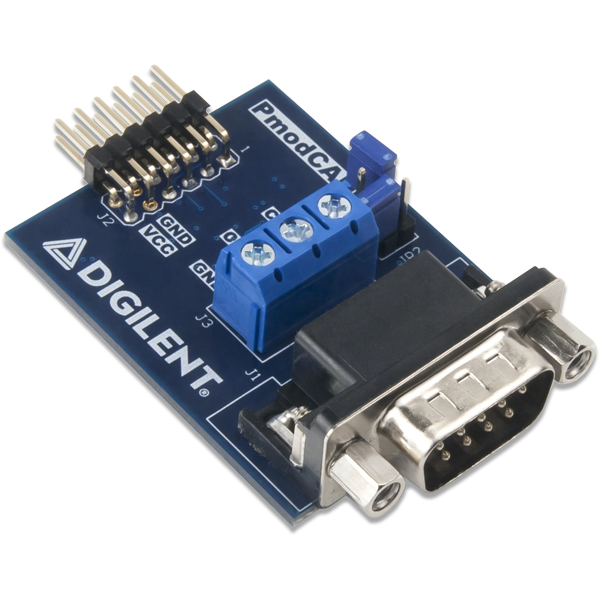
\includegraphics[width=0.5\textwidth]{./src/pmod_can.png}
        \caption{A CAN PMOD}
        \label{fig:pmod}
    \end{center}
\end{figure}
\pagebreak
\tableofcontents
\listoffigures
\listoftables
\pagebreak

\setlength{\parskip}{\medskipamount}

%------------------------------------------------------------------------------------------------------------------------------------------------------
\section{Why Should I Care?}
FPGAs enable Low Latency processing\footnote{\url{https://blog.esciencecenter.nl/why-use-an-fpga-instead-of-a-cpu-or-gpu-b234cd4f309c}}, so performing a transform on data coming in and getting the result output an be much faster than in a traditional CPU based approach. They also provide far more IO configurability than the traditional approach; the IO logic, and the pin it's connected to are totally configurable in code and constraints files\handwaving. Say a requirement changes from an 8 bit UART bus to a proprietary 11 bit UART bus - this would require a whole new microcontroller in a traditional approach however with an FPGA this might only require a change to a \texttt{generic} and a recompile. 

For the reasons stated above, typical uses of FPGAs include signal processing such as filtering\footnote{\url{https://digital-library.theiet.org/content/journals/10.1049/iet-cdt.2016.0067}}, and high speed IO such as devices produced by SpeedGoat\footnote{\url{https://www.speedgoat.com/products/simulink-programmable-fpgas-fpga-i-o-modules-io334}}.
\subsection{Toolchain}
One takeaway from this should be that toolchains are important. Each device vendor will have their own proprietary toolchain. This means that you can approach FPGA development in one of two ways:
\begin{enumerate}
    \item Choose a toolchain you're familiar with, then a device from the manufacturer
    \item Choose a device which suits your requirements, then potentially suffer with an unfamiliar toolchain
\end{enumerate}

Fortunately there are few realistic choices when it comes to this decision; use the Quartus toolchain with Intel\footnote{Altera} devices, or using the Vivado toolchain\footnote{Older Xilinx devices can use the ISE suit from Xilinx} with Xilinx devices. I am most familiar with Vivado, so this workshop is based around that. The reason for this choice is that the \emph{Zynq} range of devices from Xilinx are a System on Chip (SOC) which allows me to use either one/two ARM cores or some Programmable Logic or any combination of these in any projects I'm undertaking. Similar devices may exist from the Intel range, but at the time of buying my dev board they didn't. For an overview of some devices and toolchains you might come across see \cref{table:devices}.

\begin{table}
    \begin{center}
        \begin{tabular}{| m{4cm} | m{4cm} | m{4cm} |}
            \hline
            Manufacturer & Toolchain & Device \\ \hline
            Intel & Quartus \newline 
\includegraphics[width=30mm]{./src/quartus_logo.png} & Stratix \newline Cyclone \newline Arria \newline ... \\ \hline
            Xilinx & Vivado \newline  
\includegraphics[width=30mm]{./src/vivado_logo.jpg} & Ultrascale \newline Ultrascale+ \newline Spartan-7 \newline Virtex-7 \newline Kintex-7 \newline Artix-7 \newline Zynq-7000 \\ \hline
            Xilinx & ISE \newline 
\includegraphics[width=30mm]{./src/ise_logo.jpg} & Virtex-6 \newline Spartan-6 \newline Coolrunner CPLD \\ \hline
            ghdl & ghdl & Simulation only \\ \hline
        \end{tabular}
        \caption{An overview of devices and toolchains you might come across}
        \label{table:devices}
    \end{center}
\end{table}

There is also a third option when it comes to toolchains; if you don't care about synthesis a well known simulation tool is \texttt{ghdl}\footnote{\url{https://github.com/ghdl/ghdl}}. This allows for your VHDL code to be written, analysed, elaborated, and have testbenches run very quickly and without any synthesis. One of the obvious limitations with this is that it doesn't allow you to put the hardware onto a board. There are plenty of docs available online to reference when it comes to using this and this projects \texttt{build.sh} in the \texttt{scripts} directory might help as a starting point.  

I have seen on twitter lots of talk\footnote{\url{https://twitter.com/ico_TC}} of the ULX3S\footnote{\url{https://radiona.org/ulx3s/}}, this is a low cost Lattice based dev board but unlike most other ones mentioned it's open source, including it's toolchain consisting of \texttt{yosys, nextpnr, icestrom, iverilog, symbiflow}. NB: I haven't done much looking into this so couldn't tell you what the tools do or if they are any good, that's an \emph{exercise left for the reader}.

%------------------------------------------------------------------------------------------------------------------------------------------------------
\section{Important things to remember}
There is one main thing to remember through all of this: \textbf{It's not software it's hardware}. Everything you do should be done with the hardware you're creating in the back of your mind. You should make sure you are familiar with the design guidance for your device of choice. This is because different devices are made of different things - the Xilinx guidance, for example, states that \emph{for multiplexers greater than 64:1, the tradeoffs need to be considered}\footnote{\url{https://wiki.electroniciens.cnrs.fr/images/Xilinx_HDL_Coding_style.pdf}} anything below this the device is super quick. 


%------------------------------------------------------------------------------------------------------------------------------------------------------
\section{Finally lets get to learning about some VHDL}

\subsection{How a Module design turns into VHDL} 
In this section is an example turning from block diagram designs, into VHDL source code itself, along with an over of the data types and keywords seen in \Cref{table:keywords} and \Cref{table:datatypes}.
\subsubsection{Black Box}
Using a counter for a module, where the output \texttt{q} increments when the \texttt{clk} ticks, and the module is enabled as seen in \cref{fig:bbe}. The width of \texttt{q} is determined by the value of \texttt{data\_width}. If, for example the aim is to count up to  a \texttt{max} of 10, then \texttt{data\_width} would have to be \emph{at least} 4 wide ($\lfloor log_2(10)\rfloor + 1 = 4$). Synchronous modules in digital design also have an enable and reset inputs; allowing the user to turn it on and to put it back to a known state respectively. This can be seen as VHDL in \cref{fig:bbe_vhdl}.

\begin{figure}[H]
    \begin{center}
        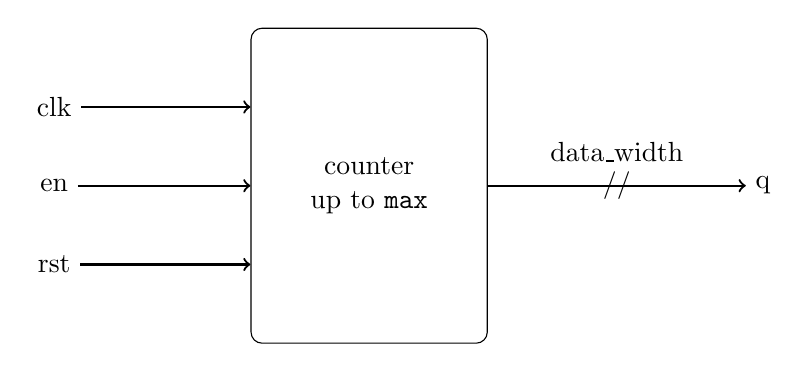
\begin{tikzpicture}[
		decoration={
      		markings,
      		mark= at position 0.5 with {\node {//};}
      	}
    ]
    \tikzstyle{entity} = [rectangle, rounded corners, minimum width=3cm, minimum height=4cm,text centered, draw=black]
    \tikzstyle{arrow} = [thick,->]
    
   
    \node (counter)[entity, align=center]{counter  \\ up to \texttt{max}};
    \node(clk)[left of=counter, xshift = -3cm, yshift=1cm]{clk};
    \node(en)[left of=counter, xshift = -3cm, yshift=0cm]{en};
    \node(rst)[left of=counter, xshift = -3cm, yshift=-1cm]{rst};
    \node (q)[right of=counter, xshift = 4cm]{q};
    \draw [arrow] (clk.east) -- ([yshift=1cm]counter.west);
    \draw [arrow] (en.east) -- ([yshift=0cm]counter.west);
    \draw [arrow] (rst.east) -- ([yshift=-1cm]counter.west);
    \draw [arrow, postaction={decorate}] (counter.east) -- node[above=5pt] {data\_width} (q.west|-counter.east);
\end{tikzpicture}
    \end{center}
    \caption{A Black Box Entity}
    \label{fig:bbe}
\end{figure}

\begin{figure}[H]
    \begin{center}
    	\lstinputlisting[language=VHDL, firstline=5, lastline=16]{../../src/counter.vhd}
    \end{center}
    \caption{A Black Box Entity in VHDL}
    \label{fig:bbe_vhdl}
\end{figure}

\subsubsection{White Box}
Now that the inputs and outputs are designed and implemented, we can look at the insides of the module. I have chosen to use a Moore Machine\footnote{\url{https://www.tutorialspoint.com/automata_theory/moore_and_mealy_machines.htm}} like in \cref{fig:mm}\footnote{\url{http://www-inst.eecs.berkeley.edu/~cs150/fa05/Lectures/07-SeqLogicIIIx2.pdf}} to do this. My implementation in \cref{fig:arch} should describe the logic diagram shown in \cref{fig:wbe}. \Cref{fig:wbe} is a system whereby the output \texttt{q} is based on the current state output only, and not the current state plus some combination of the inputs, hence it's a \emph{Moore Machine}. There is a \emph{combinatorial logic} section which works out the next thing to get clocked into the register, and a \emph{synchronous} part which clocks that through and handles the advancement of the state.

\begin{figure}[H]
    \begin{center}
        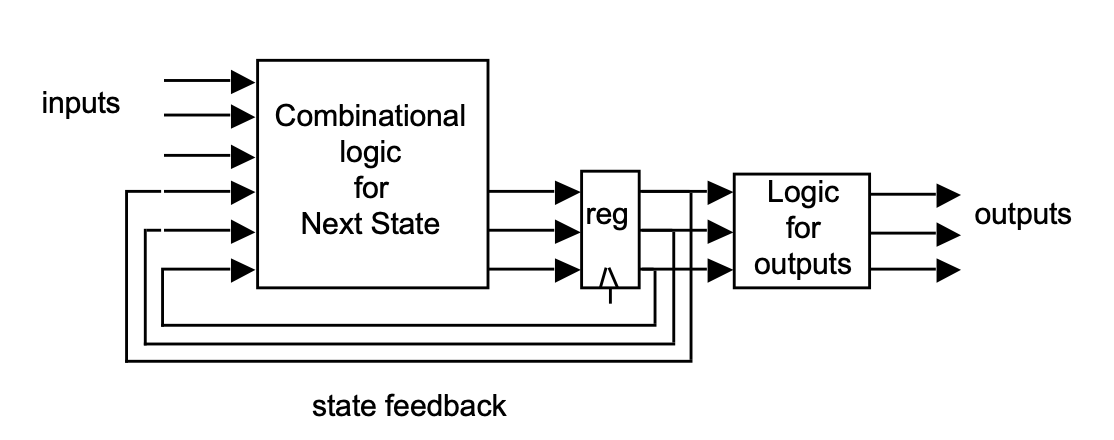
\includegraphics[width=\textwidth]{./src/moore_machine.png}
    \end{center}
    \caption{Generic Moore Machine}
    \label{fig:mm}
\end{figure}

\begin{figure}[H]
    \begin{center}
        \begin{tikzpicture}[
		decoration={
     		markings,
      		mark= at position 0.7 with {\node {//};}
      	},
      	node distance = 0.5cm
    ]
    \tikzstyle{process} = [rounded corners, minimum width=2cm, minimum height=2cm, draw=black]
    \tikzstyle{arrow} = [thick,->]            
    
    \node (SL)[process,align=left]{
    	\begin{minipage}[t][3cm]{4cm} 
    		\fontsize{8pt}{8pt}\selectfont
    		\textbf{Synchronous Logic} \\ \\ \\ 
    		\texttt{if rising edge of clock:\\\hspace*{0.25cm}if rst = '1': \\ \hspace*{0.5cm}out = 0 \\\hspace*{0.25cm}else if en = '1': \\ \hspace*{0.5cm}out = in}
    	\end{minipage}
    };
    
    \node(clk)[left = of SL, xshift=-2cm, yshift=0.9cm]{clk};
    \node(en)[left = of SL, xshift=-2cm, yshift=0.3cm]{en};
    \node(rst)[left = of SL, xshift=-2cm, yshift=-0.3cm]{rst};
    \node(Q)[right= of SL, xshift=5cm]{q};

    \node (CL)[process, align=left, below = of SL,]{
    	\begin{minipage}[t][3cm]{4cm} 
    		\fontsize{8pt}{8pt}\selectfont
    		\textbf{Combinatorial Logic} \\ \\ \\
    		\texttt{if count + 1 $\geq$ max:\\\hspace*{0.25cm}count = 0 \\ else \\\hspace*{0.25cm}count = count + 1}
    	\end{minipage}
    };
    
    \draw [arrow]  ([xshift=1cm]SL.east) |- node[below]{count} (CL.east);
    \draw [arrow] (clk.east) -- ([yshift=0.9cm]SL.west);
    \draw [arrow] (en.east) -- ([yshift=0.3cm]SL.west);
    \draw [arrow] (rst.east) -- ([yshift=-0.3cm]SL.west);
    \draw [arrow] (CL.west) -| ([xshift=-1cm]CL.west) node[ below]{count} -- ([xshift=-1cm, yshift=-0.9cm]SL.west) -- node[left, above]{in} ([yshift=-0.9cm]SL.west);
    \draw [arrow, postaction={decorate}] (SL.east) -- node[xshift=-2.3cm,above] {out} node[xshift=1cm, above=5pt] {data\_width} (Q.west|-counter.east);


	\begin{pgfonlayer}{background}
       	\path (SL.north west)+(-2,0.2) node (a) {};
		\path (CL.south east)+(+2.3,-0.2) node (b) {};
		\path[rounded corners, draw, dashed] (a) rectangle (b);
	\end{pgfonlayer}
	\end{tikzpicture}
    \end{center}
    \caption{A White Box Entity with pseudocode Moore Machine}
    \label{fig:wbe}
\end{figure}

When examining the source code in \cref{fig:arch} it important to remember that each process happens concurrently. Similarly any thing outside of a \texttt{process} block such as that on line 38 of the snippet also happens concurrently. If it helps, each line of code can be thought of as it's own process. To clarify that statement, and with reference to \cref{fig:arch}, there are 3 concurrent things happening:
\begin{enumerate}
	\item The \texttt{process} between lines 12-25, which is the \emph{combinatorial logic}
	\item The \texttt{process} between lines 27-36, which is the \emph{synchronous logic}
	\item The assignment of the output \texttt{q} on line 38
\end{enumerate}

\begin{figure}[H]
    \begin{center}
    	\lstinputlisting[language=VHDL, firstline=18]{../../src/counter.vhd}
    \end{center}
    \caption{The White Box Entity in VHDL}
    \label{fig:arch}
\end{figure}

\begin{table}[H]
    \begin{center}
    \begin{threeparttable}
        \begin{tabular}{| c | m{ 0.7\textwidth} |}
            \hline
             Keyword & Overview \\ \hline
              \texttt{process} & The start of a process, in a process each instructions happens sequentially \\ \hline
             \texttt{signal} & \handwaving Think of it as a wire that exists between processes. They are updated at the end of the process \\ \hline
              \texttt{variable} & \handwaving Variables can only exists in a process, they update immediately unlike signals \\ \hline
              \texttt{architecture} & Signifies the start of the internal details of an entity \\ \hline
              \texttt{rising\_edge}\tnote{*}& Syntactic sugar equivalent to \texttt{if clk = '1' and clk'event} \\ \hline
        \end{tabular}
        \begin{tablenotes}
        \footnotesize
        \item[*] Not really a keyword, but important to know.
        \end{tablenotes}
        \end{threeparttable}
        \caption{An overview of keywords we have seen}
        \label{table:keywords}
    \end{center}
\end{table}

\begin{table}[H]
    \begin{center}
    \begin{threeparttable}
        \begin{tabular}{| c | m{ 0.7\textwidth} |}
            \hline
             Data Type & Overview \\ \hline
              \texttt{std\_ulogic}\tnote{*}& This is defined in the \texttt{ieee.std\_logic\_1164} package and is an enumeration with the values 'U', 'X', '0', '1', 'Z', 'W', 'L', 'H' and '-' \\ \hline
              \texttt{std\_ulogic\_vector} & Again defined in the  \texttt{ieee.std\_logic\_1164} package this is an array of \texttt{std\_ulogic}s \\ \hline
             \texttt{positive} & This is a VHDL standard type and it's an \texttt{integer} with a range of 1 to at least $2^{31} -1$  \\ \hline
              \texttt{record} & This is a VHDL standard type, similar to a struct \\ \hline
        \end{tabular}
        \begin{tablenotes}
        \footnotesize
        \item[*]Many online examples use  \texttt{std\_logic}, this is the 'resolved' version of  \texttt{std\_ulogic}. They are effectively the same except a signal of type \texttt{std\_logic} can be controlled from different places and errors will only show themselves at runtime.
        \end{tablenotes}
        \end{threeparttable}
        \caption{An overview of data types we have seen}
        \label{table:datatypes}
    \end{center}
\end{table}

\subsection{Synthesiseable vs. Non-synthesiseable code}
VHDL has lots of things that can't be translated into hardware, such as the \texttt{wait} statement and files. It's important to be aware that not everything you describe can turn into hardware. If in doubt consult resources such as the \emph{Doulus Guide} in \cref{section:fa}: \nameref{section:fa}.

\subsection{How to see output from our VHDL}
There are two ways to do this
\begin{enumerate}
    \item \textbf{Simulation} - this is often the quickest method as it allows us to delve into every signal and process of our design. This also happens on our development machine so we can make great progress and do 95\% of our coding without a device. Another bonus is that it doesn't require fully synthesiseable code, so you can use \texttt{wait} statements and stuff.
    \item \textbf{Putting on the hardware} - this is where stuff gets tough. In this step the design will run at full speed on a device. You should only be doing this when you feel sufficiently confident that it'll work. If anything goes wrong here it can be extremely tough to debug it, or even detect it! It's very worthwhile having an oscilloscope\footnote{aka, DSO, silly scopes, or just scopes} at this point to help. 
\end{enumerate}

\subsubsection{Simulation}
Simulations can be stimulated via a test bench (my personal favourite) or manually in some simulators. For this tutorial I have created a testbench to do this for both the \texttt{counter} module and the \texttt{top\_model} of the design. Note that the testbenches provided don't actually do any testing, they just instantiate the modules and wait for a certain amount of time. In real life these would contain a number of \texttt{assert} and \texttt{report} statements to allow a test to automatically fail. These test benches, and the \texttt{top\_model} also give an example of structural implementation, so you can see how a module is instantiated and connected up. Simulations will pop out a waveform,  which can be quite complicated to interpret if the design is big and has loads of signal, but in the case of our counter it's pretty easy. \Cref{fig:counter_wave} shows the output of \texttt{gtkwave} where the \texttt{clk} input and the output \texttt{q} can be seen plotted, note how \emph{after} the \texttt{clk} has a rising edge the value of \texttt{q} changes.

\begin{figure}[H]
    \begin{center}
        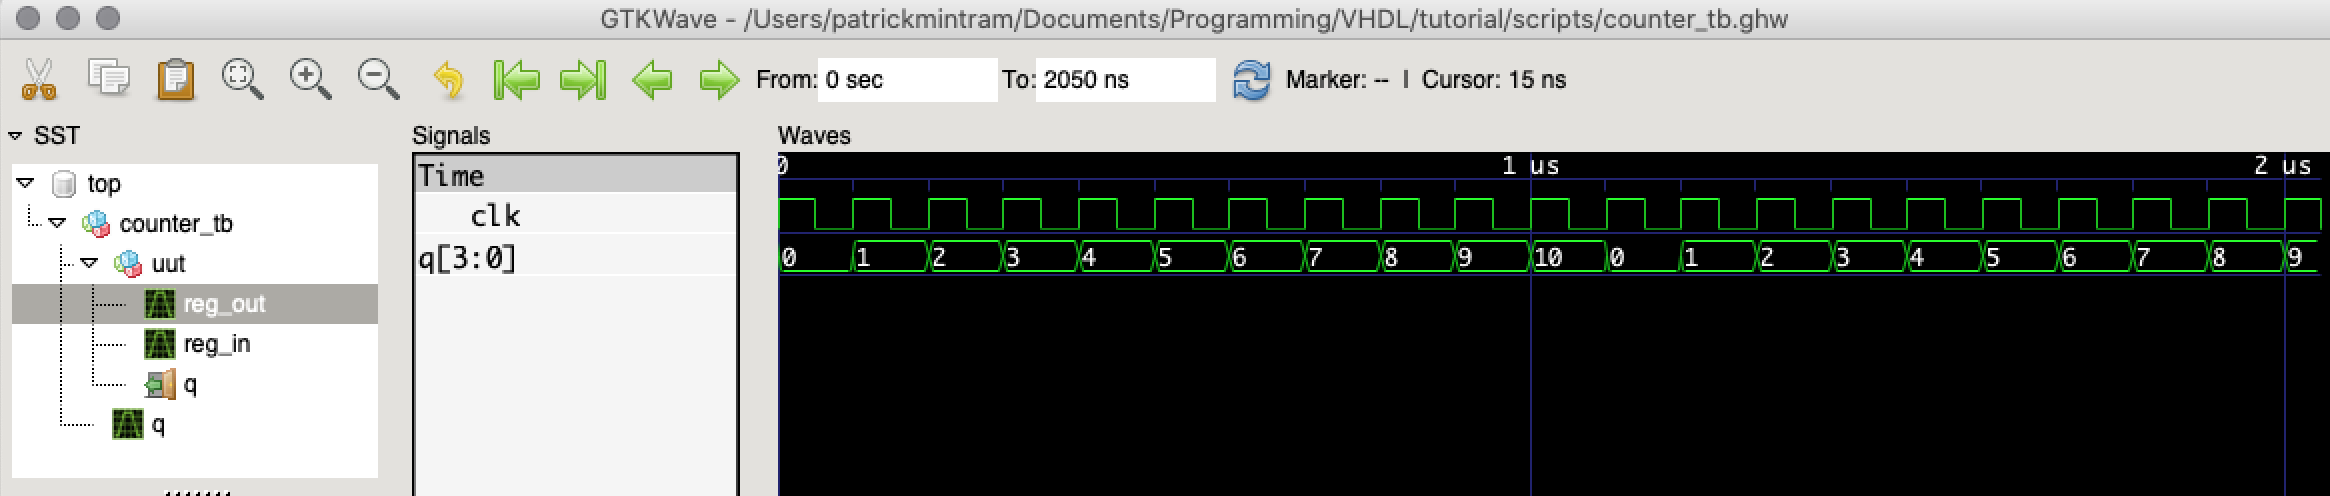
\includegraphics[width=\textwidth]{./src/counter_waveform.png}
    \end{center}
    \caption{gtkwave output of our counter}
    \label{fig:counter_wave}
\end{figure}

Although the example in \cref{fig:counter_wave} was made using \texttt{gtkwave} most waveforms generated will look the same. My advice here is to just have a play - download a simulation tool such as \texttt{ghdl} and \texttt{gtkwave}, or use the ones provided with you device's toolchain and go wild!

%------------------------------------------------------------------------------------------------------------------------------------------------------
\section{OK, now lets actually do some VHDL}\label{section:vhdl}

This section is where the majority of the instruction boxes are, as such it's very specific the to Vivado, so if you're the using a different tool at home it might not be too helpful.

\subsection{Reference Project Overview}
The reference project provided enables you to flash some LEDs at different speeds using the counter previously discussed - this demonstrates the ability to create designs with different things happening at different times and at different rates. It also contains some stubs for you to put in your own functionality; turning off and on an LED from a switch. 

\subsubsection{File Types}
A VHDL project will typically contain the following files:
\begin{enumerate}
    \item Design Source Files \texttt{*.vhd}: These contain the actual source code for the hardware you're describing. These should contain only synthesisable code.
    \item Design Test Benches \texttt{*\_tb.vhd}: These contain test benches for your design entities, usually suffixed with \texttt{\_tb} so you know it's a test bench, and will likely contain non synthesisable code.
    \item Constraints Files \texttt{*.(ucf|xcd)}: These files describe any constraints of the platform or design, such as pins used, timing requirements etc. Note that these extensions are Xilinx specific, Quartus uses \texttt{.qsd}.
    \item Scripts \texttt{*.(sh|tcl)}: These are provided to help with setting up and managing the project. \texttt{tcl} files seem to be what most tools prefer, and tools will often provide a number of utility functions to help with this. 
\end{enumerate}

\subsection{How to get started with a new design}
There are heaps of tutorials online for how to do this in all sorts of toolchains, such as this\footnote{\url{https://reference.digilentinc.com/vivado/getting_started/start}} or this\footnote{\url{https://www.intel.com/content/www/us/en/programmable/documentation/yoq1529444104707.html}} so I won't cover that here. If you're reading this and it's printed then good luck typing those in! Ask me for an electronic copy and I'll make sure you get one, alternatively google \emph{Quartus getting started} or similar.

\subsection{Open the reference project}
\subsubsection{ghdl}
This is just a command line tool, so there's no project to open. Just use vim or something to look at the files individually.

\subsubsection{Vivado}
Vivado is a pretty huge tool which produces loads of artefacts, most of which are generated by the tool so we don't need to keep them in version control. For this reason there is a \texttt{tcl} script which instructs it to setup our project again.

\instructionbox{At the terminal: \texttt{vivado -mode tcl -source tutorial.tcl}}

\subsection{Build the reference project}
\subsubsection{ghdl}
\texttt{ghdl} doesn't have an IDE or anything, so I have been using scripts to automate this build process. 

\instructionbox{\texttt{./build.sh} in the \texttt{scripts} folder}

\subsubsection{Vivado}

\instructionbox{Click \texttt{Generate Bitstream} and wait patiently, keep an eye on the top right corner of Vivado for the status!}

\subsection{Run the simulation}
\subsubsection{ghdl} 
The script you ran before already did this, if you want you can run it again.

\instructionbox{\texttt{./build.sh} in the \texttt{scripts} folder}


\instructionbox{Open it in \texttt{gtkwave}}
\\
\,
This has already been seen before in \cref{fig:counter_wave}.

\subsubsection{Vivado}

This is more complicated, because I have packaged the sources a \emph{Custom IP} so we can use it in the GUI. The easiest way of seeing the waveform is to create a new, blank, project. And to add the files in \texttt{src} and \texttt{test} as simulation sources. This isn't covered in this tutorial yet though as we are going to smash it straight on the hardware and I ran out of time.

\subsection{Load onto the Device}
In order to do this ensure you have generated the bitstream successfully. Unfortunately it's a bit of a pain, because we need to get the clock source from the ARM core working before we can see any difference in the FPGA. To do this we need to use the Vitis SDK to load an example application to the platform we have created, and run it. Fortunately this is a 'one time thing' for this practical session and we only need to do it once.

\instructionbox{In Vivado: File > Export Hardware}

\instructionbox{Open Vitis}

\instructionbox{Create Application Project}

\instructionbox{\emph{Create new platform from hardware} and nagivate to your generated \texttt{xsa} file. This is likely in your Vivado project directory}

\instructionbox{Select the \emph{Peripheral Tests} or \emph{Hello World} example project}

\instructionbox{Build}

\instructionbox{In the top toolbar select 'Run As', then double click on \emph{Single Application Debug} to create a new configuration}

\instructionbox{Click the green 'run' arrow}

\instructionbox{Play with SW0 and see LED0 turn on and off and observe the LEDs going bonkers - this is your hardware in the FPGA being clocked by the Zynq's ARM core!A


\subsection{Implement the architecture of the stubs}
Now this is up to you to choose to do something extra in the stubs provided. As a starter try:
\begin{enumerate}
	\item Make a light turn on when you move a switch to it's \emph{on} position
	\item Make a light turn on when both switches are in their \emph{on} positions
\end{enumerate}

\instructonbox{Go back to Vivado and right click the custom IP block}

\instructionbox{Select the \emph{Edit} option}

\instructionbox{Make your changes}

\instructionbox{Repackage the IP}

\instructionbox{Follow the prompts to update the IP in the block diagram}

\instructionbox{Click \emph{Generate Bitstream} again and the export the hardware}

\instructionbox{Now that the ARM's clock is ticking away we can skip the SDK and use Vivado's Hardware manager to program the device}

\subsection{Device Overview}
The Zedboard is a development board based around a Xilinx Zynq-7000 device. As previously mentioned it's got 2 ARM cores on board along with a bunch of Programmable Logic (seen in \cref{fig:zynq}). It's important to be aware of this because any bitstreams and designs we produce need to include an interface to one more more of these cores. Infact for the reference project they will serve as our clock source. There are heaps of things you can use which are already built in as peripherals to the PS such as GPIO, Serial Comms and PS-PL interuppt control. The fun part about FPGAs though is learning how to do this in the Programmable Logic!

\begin{figure}[H]
    \begin{center}
        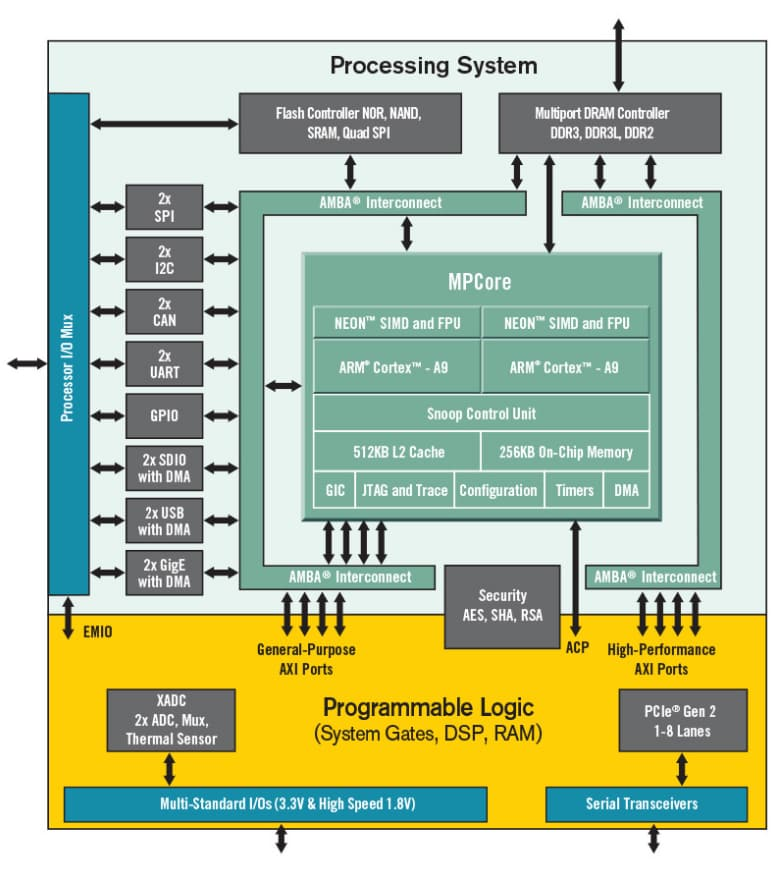
\includegraphics[width=0.7\textwidth]{./src/zynq_arch.jpg}
        \caption{The Zynq device architecture}
        \label{fig:zynq}
    \end{center}
\end{figure}

\subsubsection{How to find what connects to what}
This is an important thing to be able to do, and if you love datasheets like me you're in for a treat! First we need to identify which switches and LEDs on the physical hardware we want to use, for this I want to use slide switches 0 and 1, and LED 0. Although not marked in \cref{fig:zedoverlay} they are just above the slide switches.

\instructionbox{Find the switches and LEDs on the actual Zedboard}

\begin{figure}[H]
    \begin{center}
        \includegraphics[width=0.7\textwidth]{./src/Zedboard_Overlay.jpg}
        \caption{The Zedbaord Layout}
        \label{fig:zedoverlay}
    \end{center}
\end{figure}

The next step is to reference the schematic\footnote{Available on \url{https://www.xilinx.com}}.

\instructionbox{Find \texttt{SW0}, \texttt{SW1} and \texttt{LD0}. This can be done with a \texttt{ctrl-f} usually. These can both be found on sheet 3 of the schematic, and are shown in \cref{fig:schemled} and \cref{fig:schemsw}.}

\begin{figure}[H]
    \begin{center}
        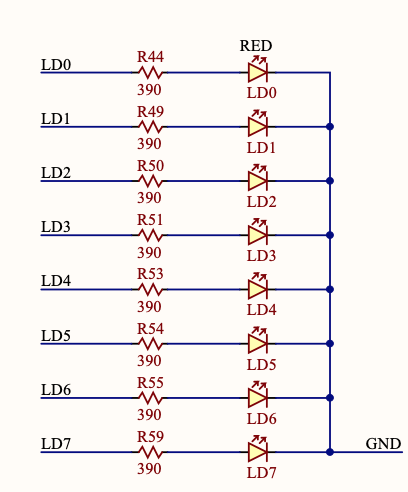
\includegraphics[width=0.4\textwidth]{./src/schem_led.png}
        \caption{The Zedboard LEDs  on the schematic}
        \label{fig:schemled}
    \end{center}
\end{figure}

\begin{figure}[H]
    \begin{center}
        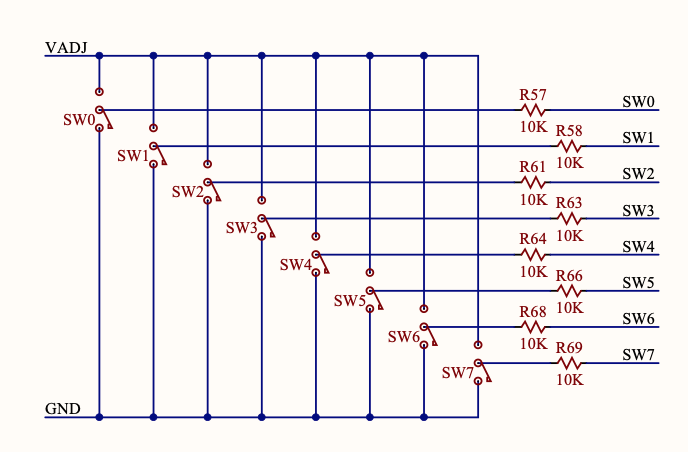
\includegraphics[width=0.5\textwidth]{./src/schem_sw.png}
        \caption{The Zedboard switches  on the schematic}
        \label{fig:schemsw}
    \end{center}
\end{figure}

On the schematic, how we have found the physical components we need to find where they connect to the FPGA BGA\footnote{Ball Grid Array - the pads attached to the FPGA IC}. This can be done by finding the other end of the \texttt{SW0} net shown on the right hand side of \cref{fig:schemsw}. It should take you to a sheet 9, and in the bottom right hand corner are the switches. Shown in \cref{fig:schembga}.


\instructionbox{Identify the BGA grid location of the connection to the FPGA}

\begin{figure}[H]
    \begin{center}
        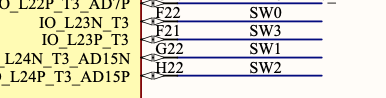
\includegraphics[width=0.5\textwidth]{./src/schem_bga.png}
        \caption{The Zedboard switches connect to the FPGA at BGA location F22 and G22}
        \label{fig:schembga}
    \end{center}
\end{figure}

%------------------------------------------------------------------------------------------------------------------------------------------------------
\section{Further Activities}\label{section:fa}
If this has been fun, and you want to learn more here are some useful resources I have had successes with:

\begin{itemize}
    \item Effective Coding with VHDL\footnote{\url{https://www.amazon.co.uk/Effective-Coding-VHDL-Principles-Practice/dp/0262034220}} 
    \item Awesome VHDL\footnote{\url{https://github.com/VHDL/awesome-vhdl}}
    \item Digital Fundamentals\footnote{\url{https://www.amazon.co.uk/Digital-Fundamentals-Thomas-L-Floyd/dp/0132737965}}
    \item Doulos Guide\footnote{\url{https://www.ics.uci.edu/~jmoorkan/vhdlref/vhdl_golden_reference_guide.pdf}}
\end{itemize}

\end{document}
